\section{Optimisation problems}
Suppose we need to choose a rectangle with a fixed perimeter, but a maximal area. By considering the
symmetry of the problem, it is almost clear that if a solution exists then it \emph{should} be a square.

Indeed, suppose that our rectangle has side lengths $ x $ and $ y $, and perimeter $ \mathcal{P} $. Then $ \mathcal{P} = 2(x + y) $,
and so the area of our rectangle (the quantity we wish to maximise) is
\begin{displaymath}
  \mathcal{A} = xy = \frac{x(\mathcal{P} - 2x)}{2} = \frac{1}{2}\mathcal{P}x - x^2.
\end{displaymath}
Noting that the graph of the function $ \mathcal{A}(x) $ is a parabola, opening downwards, it is clear
that our desired maximum is the vertex; completing the square, we find that
\begin{displaymath}
  \mathcal{A} = \frac{1}{16}\mathcal{P}^2 - \left(x - \frac{1}{4}\mathcal{P}\right)^2
\end{displaymath}
and thus the vertex has $ x$--value $ \mathcal{P}/4 $; immediately, $ x = y $ and we see that our guess,
of a square optimal shape, was correct.

We were able to solve this problem because it ended up being equivalent to finding the maximum of a quadratic,
which is easy to solve in this way with only a little effort. However, consider the following problem, which is
essentially the same but now in three dimensions:
\begin{pro}
  Find $ x $, $ y $, and $ z $, such that a rectangular prism with perimeter (sum of all 16 sides) $ \mathcal{P} $
  and surface area $ \mathcal{S} $ has maximal volume.
\end{pro}
We write $ \mathcal{P} = 4x + 4y + 4z $ and $ \mathcal{S} = 2xy + 2yz + 2zx $; considering $ V = xyz $, we substitute
in our constraints:
\begin{displaymath}
  V = x(yz) = x\left(\frac{\mathcal{S} - 2xy - 2zx}{2}\right) = \frac{1}{2}\mathcal{S}x - x^2 y - x^2 z
    = \frac{1}{2}\mathcal{S}x - x^2 (y + z) = \frac{1}{2}\mathcal{S}x - x^2 \left(\frac{\mathcal{P} - 4x}{4}\right);
\end{displaymath}
hence $ V = (\mathcal{S}/2)x - (\mathcal{P}/4)x^2 + x^3 $, and now we need to find the maximum value of a cubic --- which
is not something we can do geometrically. (Furthermore, it turns out that the `obvious' solution --- sending $ x $ to
infinity makes $ V $ tend to infinity --- does not work here, because for large enough $ x $, $ y $ and $ z $ turn out to be
undefined; the problem is actually even more interesting than this.)


Recall from Level 2 that a \emph{local maximum} of a function $ f $ is some point $ (x, f(x)) $ such that, for a sufficiently
small interval around $ x $, whenever $ y $ is in the interval then $ f(y) \leq f(x) $. A \textbf{local minimum} is defined in
a similar way. Local extrema are also sometimes called \textbf{relative extrema}.

Many optimisation problems in applied mathematics can be reduced to finding relative extrema.

\begin{exs}\leavevmode
  \begin{enumerate}
    \item The function $ x \mapsto x^2 $ has a local minimum at $ (0, 0) $.
    \item The function $ x \mapsto 2x^3 + 15x^2 + 36x + 2 $ has a local maximum at $ (-3, -25) $ and a local minimum at $ (-2, -26) $.
    \item The function $ x \mapsto \sin x $ has a local maximum at $ (2n\pi + \frac{\pi}{2}, 1) $ for every integer $ n $, and
          a local minimum at $ (2n\pi - \frac{\pi}{2}, 1) $ for every integer $ n $.
  \end{enumerate}
\end{exs}

For classification, we have the following theorem which links the location of relative extrema to the value of the derivative. Rather than
memorising the proof, you should remember the geometric idea:- the derivative is changing from a positive value to a negative value (or vice
versa), and so must pass through zero.

\begin{thm}[Fermat's theorem]
  Let $ f $ be a function; suppose $ x_0 $ is a point in the interior of the domain of $ f $, and that $ f $ has a relative extremum
  at $ (x_0, f(x_0)) $. Then $ f'(x_0) = 0 $.
\end{thm}
\begin{proof}
  Suppose $ f $ attains a relative maximum at $ x_0 $. Then for all $ h $ sufficiently close to zero, we have $ f(x_0 + h) - f(x_0) \leq 0 $.
  Hence, if $ h < 0 $, we have $ \frac{f(x_0 + h) - f(x_0)}{h} \geq 0 $ (i.e. the derivative to the left is positive) and if $ h > 0 $, we
  have $ \frac{f(x_0 + h) - f(x_0)}{h} \leq 0 $ (i.e. the derivative to the right is negative). Taking left- and right-hand limits around
  zero, we have the following chain of inequalities:
  \begin{displaymath}
    f'(x_0) = \lim_{h \to 0-} \frac{f(x_0 + h) - f(x_0)}{h} \geq 0 \geq \lim_{h \to 0+} \frac{f(x_0 + h) - f(x_0)}{h} = f'(x_0).
  \end{displaymath}
  Note that we use the fact that the derivative exists at $ x_0 $ and so the left- and right-hand limits both tend to the same value. Then the
  desired result, $ f'(x) = 0 $, follows directly.

  For a relative minimum, the proof is essentially the same but with some inequalities swapped.
\end{proof}

Motivated by this theorem, we define a \textbf{critical point} of a function $ f $ to be some value $ x $ in the domain of $ f $ such
that either $ f'(x) = 0 $, or $ f'(x) $ is undefined. In the first case, we also call the value a \textbf{stationary point}. All local
extrema occur at critical points, but not all critical points occur at extrema.

\begin{exs}\leavevmode
  \begin{enumerate}
    \item The function $ x \mapsto 2x^3 + 15x^2 + 36x + 2 $ above has critical points $ x = -2 $ and $ x = -3 $. Both of
          these are local extrema.
    \item The function $ x \mapsto x^3 $ above has a critical point at $ x = 0 $, but does not have a local extrema there.
    \item The function $ x \mapsto \frac{1}{x} $ \textit{does not} have a critical point at $ x = 0 $, \textbf{because it is not defined there}.
  \end{enumerate}
\end{exs}

\subsection*{Classifying Critical Points}
We can use the first derivative to classify extrema as either maxima or minima.
\begin{enumerate}
  \item Determine all critical points of $ f $.
  \item Determine the sign of $ f'(x) $ to the left and right of each critical point $ x_0 $:
    \begin{itemize}
      \item If $ f'(x) $ changes from positive to negative as we move from left to right across $ x_0 $, then $ f(x) $ has a local maximum at $ x_0 $.
      \item If $ f'(x) $ changes from negative to positive as we move from left to right across $ x_0 $, then $ f(x) $ has a local minimum at $ x_0 $.
      \item If $ f'(x) $ does not change sign across $ x_0 $, then $ f(x) $ does not have a relative extremum at $ x_0 $ (e.g. $ y = x^3 $).
    \end{itemize}
\end{enumerate}

On the other hand, using the second derivative, we can come up with a second test:
\begin{enumerate}
  \item Compute $ f'(x) $ and $ f''(x) $.
  \item Find all the stationary points of $ f $ by finding all the points $ x_0 $ such that $ f'(x_0) = 0 $.
  \item Determine the sign of $ f''(x) $ for each stationary point $ x_0 $:
    \begin{itemize}
      \item If $ f''(x_0) < 0 $, then $ f(x) $ has a relative maximum at $ x_0 $.
      \item If $ f''(x_0) > 0 $, then $ f(x) $ has a relative minimum at $ x_0 $.
      \item If $ f''(x_0) = 0 $, then $ f(x) $ could have a relative maximum, a relative minimum, or neither.
    \end{itemize}
\end{enumerate}

\begin{ex}
  Find and classify the critical points of $ y = x^3 - 3x^2 + 6 $.

  \textit{Solution.} We have $ \od{y}{x} = 3x^2 - 6x $ and $ \od[2]{y}{x} = 6x - 6 $. Hence
                     the critical points are $ x = 0 $ and $ x = 2 $. At the former point, $ \od[2]{y}{x} < 0 $,
                     and so the point is a maximum; at the latter point, $ \od[2]{y}{x} > 0 $ and so the point is
                     a minimum.
\end{ex}

\begin{ex}
  Find two numbers whose difference is 100 and whose product is a minimum.

  \textit{Solution.} Let the two numbers be $ x $ and $ x + 100 $. We wish to minimise $ y = x(x + 100) $;
  clearly $ y' = 2x + 100 $, and so $ x = -50 $ is a critical point. To the left of $ x = -50 $, the derivative
  is negative; to the right, the derivative is positive. Hence $ x = -50 $ is indeed a minimum. The two required
  numbers are therefore -50 and 50.
\end{ex}

\begin{ex}
  Find and classify the critical points of $ y = (x - 1)^2 + \ln x $.

  \textit{Solution.} The derivative is $ y' = 2x - 2 + \frac{1}{x} $. We therefore have one critical
  point at $ x = 0 $ (where $ y' $ is undefined); this is an asymptote.
  Setting $ y' = 0 $, we have $ 0 = 2x - 2 + \frac{1}{x} = 2x^2 - 2x + 1 $ which has no real roots. Hence $ x = 0 $ is
  the only critical point, and the curve has no local extrema.
\end{ex}

\begin{ex}
  A rectangular plot of land is to be fenced using two varieties of fence. Two opposite sides will
  use fences selling for \$3 per metre, while the other two sides will use cheaper fence selling for \$2 per metre.
  Given that the total budget is \$1200, what is the greatest area of land which can be fenced?

  \textit{Solution.} Let $ x $ be the length of one of the expensive sides; then the length of one of the cheaper
                    sides is $ \frac{1}{2}(1200 - 3x) $, and the total area is $ A = \frac{1}{2} x (1200 - 3x) = \frac{1}{2}(1200x - 3x^2) $.
                    Hence $ \od{A}{x} = 600 - 3x $. We wish to find the maximum area, so set $ \od{A}{x} = 0 $; hence $ 3x = 600 $ and $ x = 200 $.
                    Note that the second derivative is always negative, so this stationary point must be a maximum as required. The length
                    of the other side will be $ \frac{1}{2}(1200 - 600) = 300 $, and so the maximum area is $ 300 \times 200 = 60000 $ square metres.
\end{ex}

\subsection{Exercises and Problems}
\begin{enumerate}
  \item The following function is known as the \textit{logistic curve} and is used for population modelling. Find the intervals of
        concavity, and label any inflection points.
        \begin{center}
          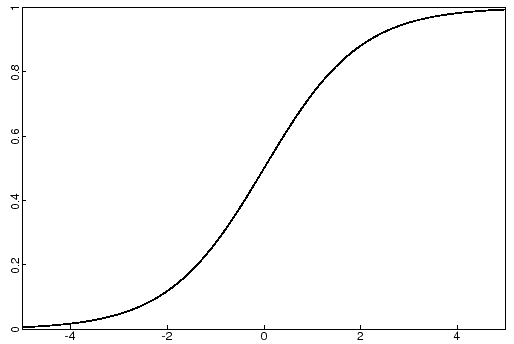
\includegraphics[width=0.4\textwidth]{logistic}
        \end{center}
  \item Find the second derivative of the following functions.
    \begin{enumerate}
      \item $ y = x^2 + x $
      \item $ f(x) = \sin x $
      \item $ g(x) = \cot(3x^2 + 5) $
      \item $ y = \frac{\sin mx}{x} $
      \item $ y = 4 \sin^2 x $
      \item $ y = \tan^2 (\sin \theta) $
      \item $ y = \tan \sqrt{1 - x} $
    \end{enumerate}
  \item Find the concavity of the function $ y = \frac{x^2 - 1}{x^2 + 1} $ at $ (0, -1) $.
  \item Find the intervals on which the following functions are increasing or decreasing, and
        find their intervals of concavity.
    \begin{enumerate}
      \item $ y = x^2 + 1 $
      \item $ y = 2x^3+ 3x^2 - 36x $
      \item $ G(x) = x - 4\sqrt{x} $
    \end{enumerate}
  \item The graph of $ y = f(x) $ (where $ f $ is a continuous function) is concave up for all $ x < 0 $, concave down for $ x > 0 $, and decreasing everywhere.
    \begin{enumerate}
      \item Sketch the graph of $ y = f(x) $.
      \item What can you say about $ f'(x) $ and $ f''(x) $ for $ x < 0 $ and $ x > 0 $?
      \item What about $ x = 0 $?
    \end{enumerate}
  \item Find a value of $ k $ such that the function $ F $ is continuous at $ x = -3 $, where
        \begin{displaymath}
          F(x) =
          \begin{cases}
            \frac{x^2 - 9}{x+3} & \text{if } x \neq -3,\\
            k                   & \text{if } x = -3.
          \end{cases}
        \end{displaymath}
  \item Show whether or not the function $ g $ is continuous at the three points $(2, g(2)) $, $ (3,g(3)) $, and  $(4,g(4)) $, where
        \begin{displaymath}
          g(x) =
          \begin{cases}
            2x-x^2              & \text{if } 0 \leq 2,\\
            2-x                 & \text{if } 2 < x \leq 3,\\
            x-4                 & \text{if } 3 < x \leq 4,\\
            \pi                 & \text{if } x \geq 4.
          \end{cases}
        \end{displaymath}
  \item Find all values of $ \alpha $ such that $ \Phi $ is continuous everywhere, where
        \begin{displaymath}
          \Phi(x) =
          \begin{cases}
            x+1                 & \text{if } x \leq \alpha, \\
            x^2                 & \text{if } x > \alpha.
          \end{cases}
        \end{displaymath}
  \item Sketch a function satisfying the given criteria.
    \begin{enumerate}
      \item
        \begin{itemize}
          \item Vertical asymptote at $ x = 0 $,
          \item $ f'(x) > 0 $ if $ x < -2 $,
          \item $ f'(x) < 0 $ if $ x > -2 $ ($ x \neq 0 $),
          \item $ f''(x) < 0 $ if $ x < 0 $, $ f''(x) > 0 $ if $ x > 0 $.
        \end{itemize}
      \item
        \begin{itemize}
          \item $ f'(0) = f'(2) = f'(4) = 0 $,
          \item $ f'(x) > 0 $ if $ x < 0 $ or $ 2 < x < 4 $,
          \item $ f'(x) < 0 $ if $ 0 < x < 2 $ or $ x > 4 $,
          \item $ f''(x) > 0 $ if $ 1 < x < 3 $,
          \item $ f''(x) < 0 $ if $ x < 1 $ or $ x > 3 $.
        \end{itemize}
    \end{enumerate}
  \item A curve is defined by the function $ f(x) = e^{-(x-k)^2} $. Find, in terms of $ k $, the $ x$-ordinates for which $ f''(x) = 0 $.
  \item It turns out that if a function $ f $ is differentiable at $ a $ then $ f $ is always continuous at $ a $, but the converse
        is not true: there exist continuous functions that are not differentiable. (In fact, there exist functions that are continuous
        everywhere but differentiable nowhere.) \label{exercise:contnotdif}
    \begin{enumerate}
      \item We will prove that differentiability of $ f $ at $ a $ implies continuity of $ f $ at $ a $; expand the following
            and use the limit laws to show that $ \lim_{x \to a} f(x) - f(a) = 0 $, carefully indicating where you use the existence
            of the derivative.
            \begin{displaymath}
              \left[\lim_{a \to x} f(x) - f(a)\right]\left[\lim_{a \to x} \frac{x - a}{x - a}\right]
            \end{displaymath}
      \item Give an example of a function which is continuous but not differentiable at some point.
    \end{enumerate}
  \item We will do some studies of convexity that may be familiar to students who have looked at the exercises on convexity
        in the algebra notes. We assume that all functions are continuous and differentiable everywhere for simplicity.
    \begin{enumerate}
      \item Show that if $ f $ is a convex function, and if $ P = (p,f(p)) $ and $ Q = (q,f(q)) $ are any two distinct points
            on the graph of $ f $, then for every point $ X = (x_1, x_2) $ on the line segment $ \overline{PQ} $, $ x_2 \geq f(x_1) $
            and equality is only obtained at the endpoints.
      \item Show that if $ f $ is a convex function, and if $ P = (p,f(P)) $ is a point on the graph of $ f $, then for every
            point $ (x_1,x_2) $ on the tangent line to $ f $ at $ P $, $ x_2 \leq f(x_1) $ and equality is only obtained at $ P $.
      \item Prove similar statements to (a) and (b) in the case that $ f $ is a concave function. [Hint: there is not much work
            involved, as long as one ponders the function $ -f $.]
    \end{enumerate}
  \item Scholarship 2010: Recall that the points of inflection of a curve are places where the second derivative
        changes sign. These are typically, \textbf{but not always}, points at which the second derivative is zero.

        Consider the curve $ y = \sqrt[3]{x} e^{-x^2} $.

        Write the second derivative in the form $ \od[2]{y}{x} = (ax^4 + bx^2 + x)e^{-x^2} x^{-5/3} $, and hence
        find the $ x$-ordinates of the points of inflection of the curve.
  \item Scholarship 2004: (You may wish to remind yourself how to perform long division of polynomials.) Consider the function
        \begin{displaymath}
          y = \frac{x^2}{1 + x^2},
        \end{displaymath}
        where $ -1 \leq x \leq 1 $. The gradient at the point $ x = 1 $ is $ \frac{1}{2} $.

        Hence show that there is a point with $ \frac{1}{4} \leq x \leq \frac{1}{2} $ where the gradient is also $ \frac{1}{2} $.
  \item Scholarship 2013: A function $ f $ is \textbf{even} if $ f(-x) = f(x) $ for all $ x $ in its domain, and \textbf{odd} if $ f(-x) = f(-x) $
        for all $ x $ in its domain.
    \begin{enumerate}
      \item Describe which polynomials are even, which are odd, and which are neither.
      \item Suppose that $ g $ is any even differentiable function defined for all real numbers (not necessarily a polynomial). Use the
            limit definition of the derivative to prove that $ g' $ is odd.
    \end{enumerate}
  \item Recall that we can define the derivative of $ f $ by $ \mathsf{D}f(x) = \lim_{y \to x} \frac{f(y) - f(x)}{y - x} $.
        We will generalise this, by writing $ \mathsf{SD}f(x) = \lim_{h \to 0} \frac{f(x + h) - f(x - h)}{2h} $.
        This is called the \emph{symmetric derivative} of $ f $.
    \begin{enumerate}
      \item In fact, we defined the derivative of $ f $ at $ x $ to be the unique $ f' $ such that $ f(x + h) \approx f(x) + hf'(x) $
            for small $ h $.\footnote{Then we defined the notation $ \varphi(x,h) \approx \psi(x,h) $ to mean that $ \varphi(x) = \psi(x) + \vartheta(h) $
            for some function $ \vartheta $ satisfying $ \vartheta(h)/h \to 0 $ as $ h \to 0 $.}

            Show that, for small $ h $, if $ f'(x) $ exists then $ f(x + h) - f(x - h) \approx 2hf'(h) $. Hence
            conclude that $ \mathsf{SD}f(x) = \mathsf{D}f(x) $ whenever the latter exists.
      \item The converse is not true: show that if we define $ f(x) = \abs{x} $, then $ \mathsf{SD} f(0) $ exists
            but $ \mathsf{D} f(0) $ does not.
      \item Define the \emph{second} symmetric derivative of $ f $ by
            \begin{displaymath}
              \mathsf{SD}^2 f(x) = \lim_{h \to 0} \frac{\frac{f(x + h) - f(x)}{h} - \frac{f(x) - f(x - h)}{h}}{h} = \lim_{h \to 0} \frac{f(x + h) - 2f(x) + f(x - h)}{h^2}.
            \end{displaymath}
            Show that whenever $ f''(x) = \mathsf{D}^2 f(x) $ exists then $ \mathsf{SD}^2 f(x) $ exists and has the same value; show that the converse
            does not hold (i.e. the existence of the second symmetric derivative does not imply the existence of the usual second derivative)
            by considering a suitable function, such as
            \begin{displaymath}
              \mathrm{sgn}(x) = \begin{cases} -1 & x < 0 \\ 0 & x = 0 \\ 1 & x > 0. \end{cases}
            \end{displaymath}
    \end{enumerate}
  \item One may recall from one of the L1 externals that we can recover a quadratic equation given a table of its values. Suppose
        we know that the following table gives points on the graph of $ f(x) = ax^2 + bx + c $.

        \begin{tabular}{c|c}
          $ x $ & $ f(x) $ \\
          $ 0 $ & $ -5 $ \\
          $ 1 $ & $ 2 $ \\
          $ 2 $ & $ 15 $
        \end{tabular}

        Define the \emph{discrete first and second derivatives} of $ f $ by $ \Delta f(x) = f(x + 1) - f(x) $ and $ \Delta^2 f(x) = \Delta f(x + 1) - \Delta f(x)  $.
        According to the god-given material in L1, we know that if $ f $ is a quadratic, then $ a = \frac{1}{2} \Delta^2 f(x) $ (for any choice of $ x $); in this
        example, we can fill in the table as follows:-

        \begin{tabular}{c|c|c|c}
          $ x $ & $ f(x) $ & $ \Delta f(x) $ & $ \Delta^2 f(x) $\\
          $ 1 $ & $ -5 $ & $ 7 $ & $ 6 $\\
          $ 2 $ & $ 2 $ & $ 13 $ & \\
          $ 3 $ & $ 15 $ &&
        \end{tabular}

        Hence $ a = 3 $. We can then write (since we know $ f $ is a quadratic) $ bx + c = f(x) - 3x^2 $, which tells us that $ b\cdot 1 + c = -8 $
        and $ b \cdot 2 + c = -10 $; hence $ b = (-10 - {}^{-}8)/1 = -2 $ and $ c = -6 $. \label{exercise:funtimeswithcalculus}

        \begin{enumerate}
          \item Justify the above steps. (Possible approach: $ hf''(x) \approx f'(x + h) - f'(x) $; set $ h = 1 $, and work out what fudge
                factor $ \vartheta(h) $ we have.)
          \item Develop a theory of discrete first and second derivatives. (Possible routes of study could include: finding a geometric
                meaning of the discrete derivatives; defining discrete $ n$th derivatives; studying the relationship between the discrete
                derivatives and the usual derivatives. You may also want to generalise my definition: instead of $ f(x + 1) - f(x) $,
                perhaps one might like to look at $ [f(x + k) - f(x)]/k $ (sans limit).)
        \end{enumerate}
  \item These problems relate to the optional section on curvature and arc length.
    \begin{enumerate}
      \item If $ y = f(x) $, formula \ref{eqn:sbyx} gives us the derivative of arc length with respect to distance
            along the $ x$-axis. What is the arc length along the graph of the function $ f(x) = \frac{1}{3}x^3 - x $
            between the vertical lines $ x = 0 $ and $ x = 5 $?
      \item Repeat (a) for the function $ g(x) = \ln \abs{\sec x} $.
      \item What is the curvature of a straight line?
      \item Calculate the curvature $ \kappa(x) $ of the function $ f(x) = x^2 $ at the points $ x = 0 $, $ x = 2 $, and $ x = 4 $.
            Draw the osculating circles at each of these points. What happens to $ \kappa(x) $ as $ x \to \infty $?
    \end{enumerate}
  \item Define $ f $ by
        \begin{displaymath}
          f(x) = \begin{cases} e^{-1/x^2} & x \neq 0 \\ 0 &x = 0 \end{cases}.
        \end{displaymath}
    \begin{enumerate}
      \item Show that $ f $ is differentiable at zero.
      \item Show that, for all $ n > 0 $, $ f^{(n)}(0) = 0 $. (Implicit here is the existence of the $ n$th derivative.)
      \item Show that $ f $ has a global minimum at zero.
      \item Justify that there can thus never be a rule, based simply on checking $ n$th derivatives, for proving
            that any function has a local minimum or maximum at a point.
      \end{enumerate}
\end{enumerate}

\subsection{References}
A good introduction to the geometry of curves, and differential geometry in general, is \emph{Differential Geometry
of Curves and Surfaces} by Manfredo P. do Carmo.

For a discussion of the history of continuity, see J F Harper (2016): Defining continuity of
real functions of real variables, BSHM Bulletin: Journal of the British Society for the History
of Mathematics, DOI:10.1080/17498430.2015.1116053 (\url{http://homepages.ecs.vuw.ac.nz/~harper/harper16.pdf}).

Discrete derivatives (see exercise \ref{exercise:funtimeswithcalculus}) are useful when taking
derivatives numerically (say we have a table of numbers defining a function $ f $, but we don't
have a nice formula for it). The kinds of things one may want to search for in a library catalogue
are ``difference calculus'' or ``discrete calculus''.

\subsection{Homework}
\paragraph{Reading}
\begin{figure}
  \centering
  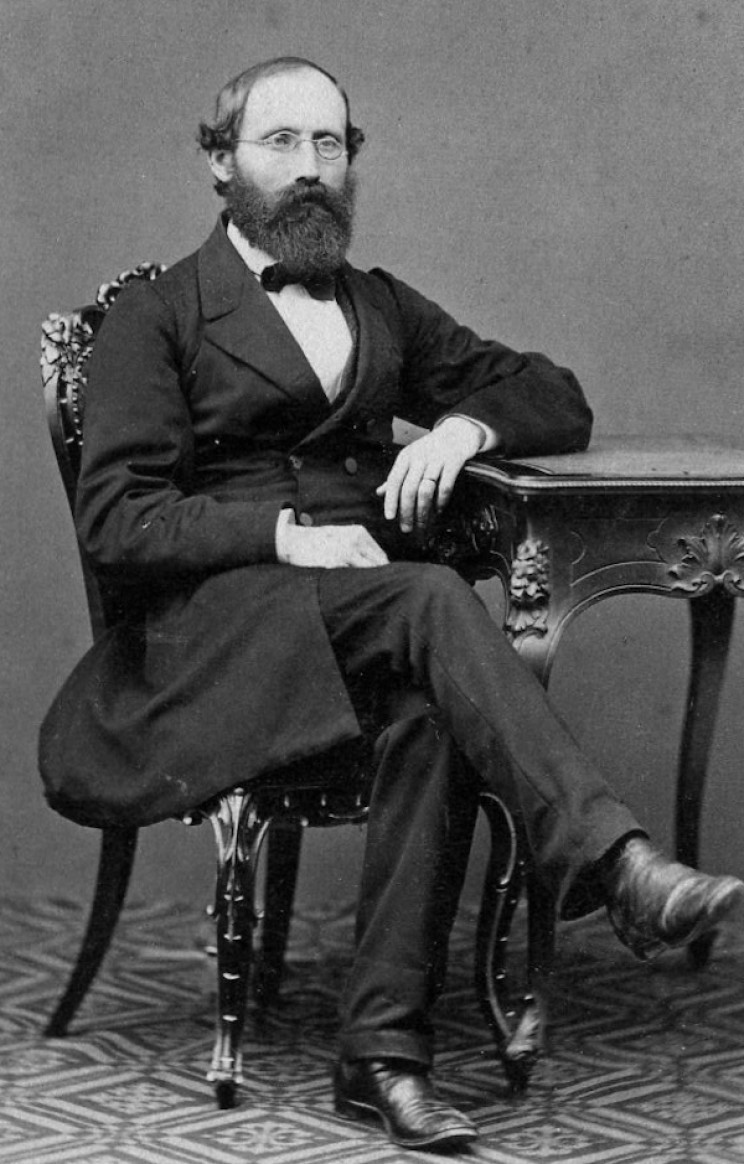
\includegraphics[width=0.2\textwidth]{riemann}
  \caption{Bernhard Riemann (public domain)}
\end{figure}
Bernhard Riemann (born September 17, 1826, Breselenz, Hanover [Germany] --- died July 20, 1866, Selasca, Italy) was a German mathematician whose profound and novel approaches to the study of geometry laid the mathematical foundation for Albert Einstein's theory of relativity. He also made important contributions to the theory of functions, complex analysis, and number theory.

Riemann was born into a poor Lutheran pastor's family, and all his life he was a shy and introverted person. He was fortunate to have a schoolteacher who recognized his rare mathematical ability and lent him advanced books to read, including Legendre's \textit{Number Theory} (1830). Riemann read the book in a week and then claimed to know it by heart. He went on to study mathematics at the University of Göttingen in 1846--47 and 1849--51 and at the University of Berlin (now the Humboldt University of Berlin) in 1847--49. He then gradually worked his way up the academic profession, through a succession of poorly paid jobs, until he became a full professor in 1859 and gained, for the first time in his life, a measure of financial security. However, in 1862, shortly after his marriage to Elise Koch, Riemann fell seriously ill with tuberculosis. Repeated trips to Italy failed to stem the progress of the disease, and he died in Italy in 1866.

Riemann's visits to Italy were important for the growth of modern mathematics there; Enrico Betti in particular took up the study of Riemannian ideas. Ill health prevented Riemann from publishing all his work, and some of his best was published only posthumously --- e.g., the first edition of Riemann's \textit{Gesammelte mathematische Werke} (1876; ``Collected Mathematical Works''), edited by Richard Dedekind and Heinrich Weber.

In 1854 Riemann presented his ideas on geometry for the official postdoctoral qualification at Göttingen; the elderly Gauss was an examiner and was greatly impressed. Riemann argued that the fundamental ingredients for geometry are a space of points (called today a manifold) and a way of measuring distances along curves in the space. He argued that the space need not be ordinary Euclidean space and that it could have any dimension (he even contemplated spaces of infinite dimension). Nor is it necessary that the surface be drawn in its entirety in three-dimensional space. A few years later this inspired the Italian mathematician Eugenio Beltrami to produce just such a description of non-Euclidean geometry, the first physically plausible alternative to Euclidean geometry. Riemann's ideas went further and turned out to provide the mathematical foundation for the four-dimensional geometry of space-time in Einstein's theory of general relativity. It seems that Riemann was led to these ideas partly by his dislike of the concept of action at a distance in contemporary physics and by his wish to endow space with the ability to transmit forces such as electromagnetism and gravitation.

\begin{flushright}
  Adapted from \textit{Bernhard Riemann} (by Jeremy John Gray) in the Encyclopaedia Britannica, \url{https://www.britannica.com/biography/Bernhard-Riemann}.
\end{flushright}

\paragraph{Problems}
\begin{enumerate}
  \item Explain, with sketches, the geometric meaning of the second derivative.
  \item Find the second derivative of the following functions.
    \begin{enumerate}
      \item $ f(x) = x^5 - 5x + 3 $
      \item $ f(x) = \frac{x^2}{x - 1} $
      \item $ f(x) = \sqrt{x} - \sqrt[4]{x} $
    \end{enumerate}
  \item Sketch a function satisfying the given criteria.
    \begin{enumerate}
      \item (hint: your result should be an odd function)
        \begin{itemize}
           \item $ f'(1) = f'(-1) = 0 $,
           \item $ f'(x) < 0 $ if $ \abs{x} < 1 $,
           \item $ f'(x) > 0 $ if $ 1 < \abs{x} < 2 $,
           \item $ f'(x) = -1 $ if $ \abs{x} > 2 $.
        \end{itemize}
      \item
        \begin{itemize}
          \item $ f'(x) < 0 $,
          \item $ f''(x) < 0 $.
        \end{itemize}
    \end{enumerate}
\end{enumerate}
